\documentclass[12pt]{article}

% Packages for math and formatting
\usepackage{amsmath}
\usepackage{amssymb}
\usepackage{amsthm}
\usepackage{geometry}
\usepackage{fancyhdr}
\usepackage{graphicx}
\usepackage{setspace}
\usepackage{listings}
\usepackage{xcolor}

\lstset{ %
    language=Matlab,                % 语言选择
    basicstyle=\ttfamily\small,     % 字体样式和大小
    keywordstyle=\color{blue},      % 关键字的颜色
    commentstyle=\color{gray},      % 注释的颜色
    stringstyle=\color{red},        % 字符串的颜色
    numbers=left,                   % 行号位置 (左侧)
    numberstyle=\tiny\color{gray},  % 行号的样式
    stepnumber=1,                   % 行号增量
    numbersep=5pt,                  % 行号与代码的距离
    backgroundcolor=\color{white},  % 背景色
    showspaces=false,               % 不显示空格符
    showstringspaces=false,         % 不显示字符串中的空格符
    showtabs=false,                 % 不显示制表符
    frame=single,                   % 给代码加上边框
    tabsize=4,                      % 设置制表符宽度
    captionpos=b,                   % 标题位置
    breaklines=true,                % 自动换行
    breakatwhitespace=true,         % 只在空格处换行
    title=\lstname,                 % 显示代码名称
    escapeinside={\%*}{*)},         % 在代码中加入LaTeX指令
    morekeywords={*,...}            % 自定义更多关键词
}

\setstretch{1.2}
\setlength{\parskip}{1em}

% Geometry settings for better margins
\geometry{a4paper, margin=1in}

% Header and footer
\pagestyle{fancy}
\fancyhf{}
\fancyhead[L]{Kecai Xuan}
\fancyhead[C]{Math Homework}
\fancyhead[R]{\today}
\fancyfoot[C]{\thepage}

% Custom commands for common math symbols
\newcommand{\R}{\mathbb{R}}
\newcommand{\N}{\mathbb{N}}
\newcommand{\Z}{\mathbb{Z}}

\begin{document}

\setlength{\parindent}{0pt}

\title{AMSC660 Homework \#12}
\author{Kecai Xuan}
\date{\today}
\maketitle

\section*{Task 1}

The number of misclassified digits first rises up when PCA components increases, and then decreases. The optimal number of PCA components is around 30, which gives the lowest number of misclassified digits.

\begin{figure}[ht]
    \centering
    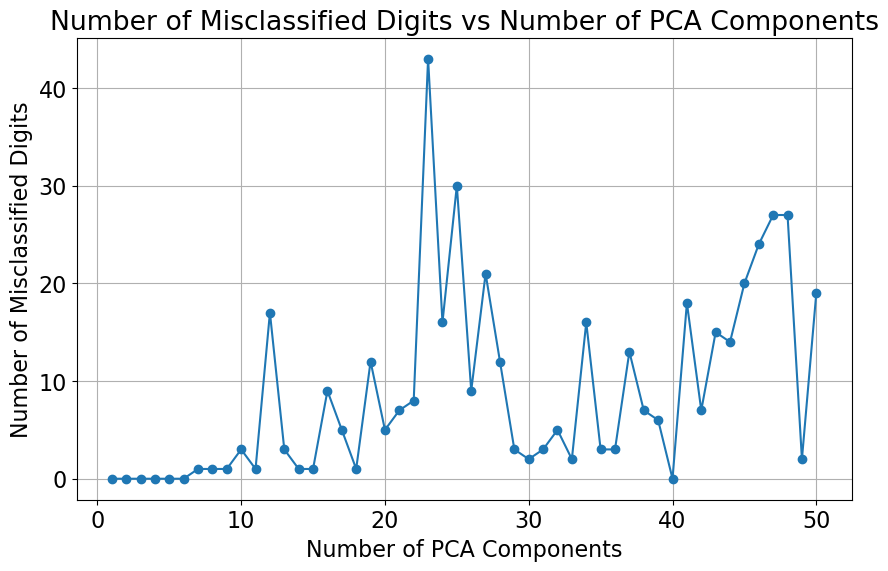
\includegraphics[width=0.6\textwidth]{./imgs/component.png}
\end{figure}

This is the learning curves when number of PCA components equals to 25:
\begin{figure}[ht]
    \centering
    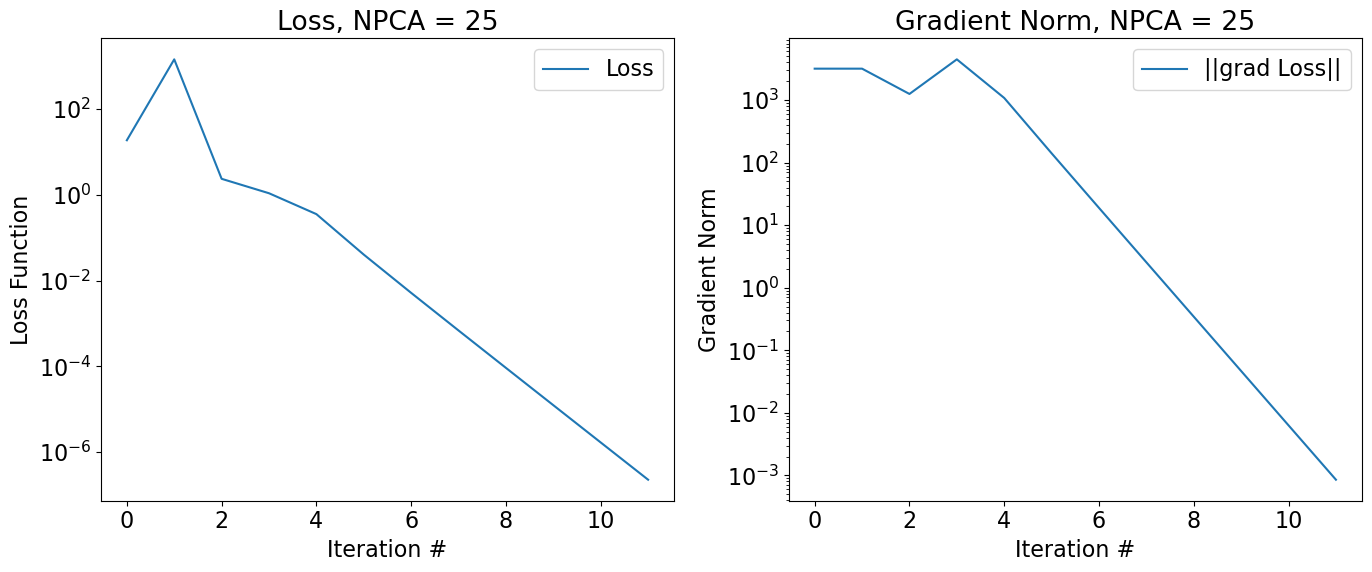
\includegraphics[width=0.82\textwidth]{./imgs/loss.png}
\end{figure}


\section*{Task 2}

This is the learning curves when using Gauss-Newton method:
\begin{figure}[ht]
    \centering
    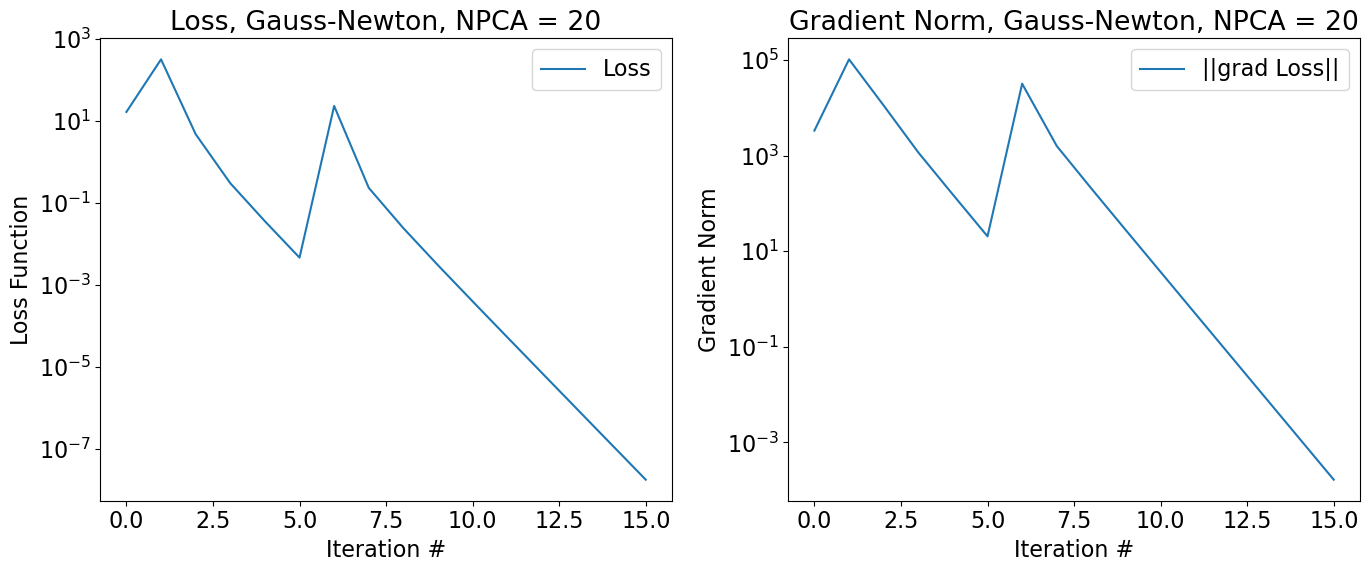
\includegraphics[width=0.82\textwidth]{./imgs/gauss_newton.png}
\end{figure}


\section*{Task 3}



\end{document}
